\documentclass[a4paper,10pt]{article}
\usepackage[utf8]{inputenc}
\usepackage{amsmath}
\usepackage{tabularx}
\usepackage{graphicx}
\usepackage{epstopdf}
\usepackage{textcomp}
\usepackage{amsmath}
\usepackage{float}
\usepackage{listings}             % Include the listings-package

\newcolumntype{b}{X}
\newcolumntype{s}{>{\hsize=.25\hsize}X}

%opening
\title{Informe técnico: \\
Placas de adquisición}
\author{P. Domenichini, A. Mendez -- Grupo 8}

\begin{document}

\maketitle

\begin{abstract}
    En el presente informe se estudiaron las capacidades de dos placas de adquisición. Las placas utilizadas fueron un sensor  {\sc daq} y un arduino  {\sc uno}. 
\end{abstract}

\section{Sensor DAQ}

Se utilizó una placa de adquisición DAQ-Vernier de la marca National Instruments. Las capacidades de adquisición se estudiaron mediante los puertos 11 ($V1$), 10 ($V2$) y 9 ($Ground$) de esta. La lectura de datos se realizó con {\sc python}, implementando el módulo {\sc nidaqmx.system}. A continuación se detalla el código utilizado con tal fin:
\lstset{language=Python}
\begin{lstlisting}[frame=single]  % Start your code-block

import nidaqmx.system

wave=[]
rate = 1000
with nidaqmx.Task() as task:
    task.ai_channels.add_ai_voltage_chan("Dev8/ai0")
    task.timing.cfg_samp_clk_timing(rate=rate)
    wave=task.read(number_of_samples_per_channel=rate)
\end{lstlisting}
La tasa de muestreo "rate" se definió igual a 1000 en todas las mediciones. 

Las respuestas en voltaje y frecuencia de la placa se muestran en la Figura~1 (a), (b), y (c), respectivamente. La amplitud mínima (panel a) es menor a 20 m$V_{pp}$, siendo ésta la mínima que se puede obtener con el generador de ondas utilizado. En el panel b, se puede observar que la amplitud máxima de voltaje es $\pm 10 V_{pp}$.  La caracterización en frecuencia se resume en el panel c. La frecuencia máxima registrada fue de 1kHz, la cual se corresponde a la tasa de muestreo preestablecida. No se realizaron mediciones con valores mayores a 1000. 
Además, se evaluó la capacidad de la placa para medir en simultáneo. Para esto, se envió una rampa en ambos canales, y se midió la  diferencia entre ellos ($\Delta V$). La conexión realizada se puede ver en la Figura 2a. El valor medido de $\Delta V$ resultó distinto de cero (ver Figura 2c), de manera que ambos canales tienen una diferencia temporal en la adquisión. 

Para la determinación de la diferencia temporal entre los canales de la placa DAQ, se procedió de la siguiente manera. Se consideraron dos rampas, las cuales fueron aproximadas como rectas:

\begin{equation*}
    V_{1} = A \cdot t + V0_1
\end{equation*}
\begin{equation*}
    V_{2} = A \cdot t + V0_2
\end{equation*}

Siendo $A$ la pendiente de la rampa; $t$ el tiempo; y $V0_{1,2}$ los voltajes iniciales de los canales 1 y 2, respectivamente.
El valor de $A$ se determinó utilizando la Configuración 1 de la Figura 2a. Los resultados obtenidos fueron ajustados mediante una recta, como se muestra en la Figura 2b. Por conveniencia tomamos $V0_1$ igual a $0$, y $V_2$ se calculó a partir de la medida realizada con la Configuración 2. Se colectaron datos durante 1 segundo, y se realizó un histograma (ver Figura 2d). La distribución obtenido fue ajustada con una función gaussiana, obteniéndose el valor medio y su dispersión, cómo se muestra con línea sólida en la Figura 2d. El tiempo de defasaje entre ambos canales ($t_{def}$) se calculó como:
\begin{equation*}
    -V0_{2} = A \cdot t_{def} \Rightarrow t_{def} = \frac{- V0_{2}}{A}
\end{equation*}
Los resultados obtenidos fueron $A=(0.1608 \pm 0.0001) \frac{V}{s}$, $V0_2 = -(0.003 \pm 0.001) V$, y $t_{def} = (0.019 \pm 0.006)s$.

\begin{figure}[H]
  \centering
  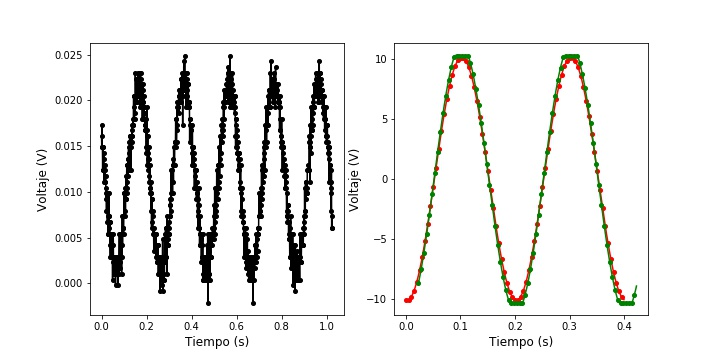
\includegraphics[width=0.8\textwidth]{DAQ_amplitud.jpg} \\
  (a) \hspace{4cm} (b)
  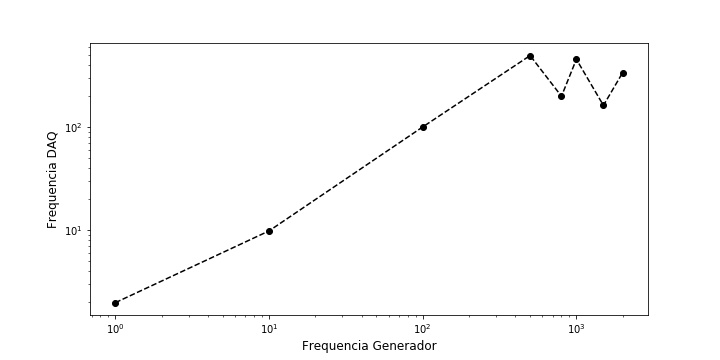
\includegraphics[trim={0 0 0 1.cm},clip, width=0.8\textwidth]{DAQ_logfrequency.jpg}
  (c)
  \caption{Respuesta en amplitud (a) mínima, (b) máxima, y (c) en frecuencia de la placa DAQ.}
  \label{fig:resp_freq}
\end{figure}

\begin{figure} [H]
    \centering
    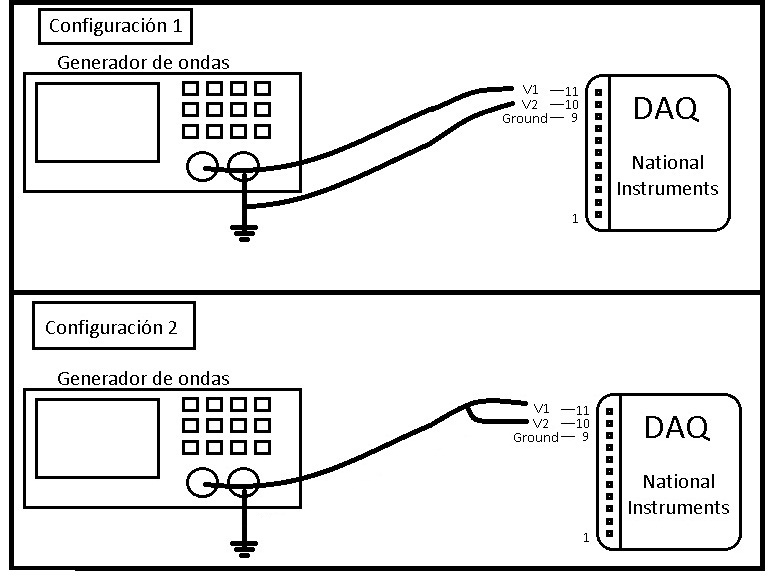
\includegraphics[width=0.4\textwidth]{DAQ-configuraciones.jpg} (a)
    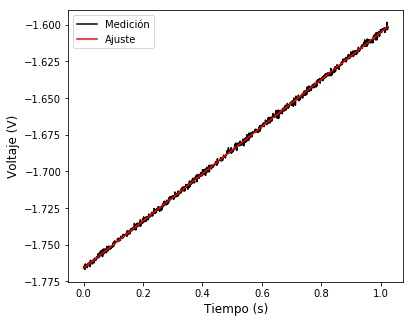
\includegraphics[width=0.4\textwidth]{ajustelineal.jpg} (b) \\
    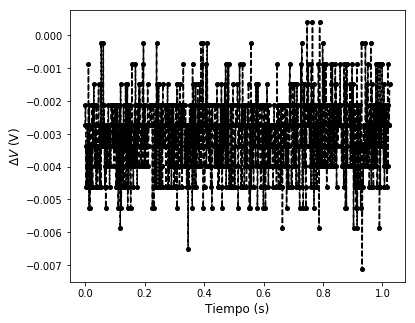
\includegraphics[width=0.4\textwidth]{diferencia.jpg} (c) 
    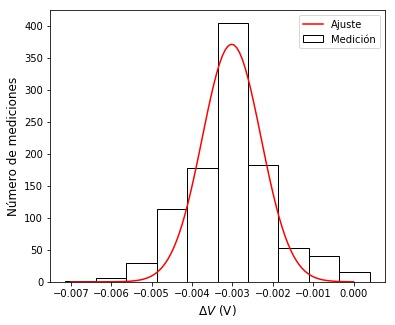
\includegraphics[width=0.4\textwidth]{histogramafit.jpg} (d)
    \caption{(a) Configuraciones utilizadas para medir una señal (1) y una diferencia (2). (b) Medida de la señal de la rampa utilizada. 
    (c) Medida de la diferencia de los canales mandando una rampa de voltajes. (d) Histograma de las medidas obtenidas de $\Delta V$. }
    \label{fig:diffV}
\end{figure}

Finalmente, los valores de respuesta en amplitud y frecuencia de la placa DAQ se resumen en la Tabla~1.
\begin{table}[h]
\begin{tabularx}{\textwidth}{b|s|s|s }
Característica & Min & Máx & Unidad \\
\hline
Voltaje señal de entrada & 10 & -10 & V \\ 
Frecuencia señal de entrada & 1 & 10000 & Hz \\
\end{tabularx}
\label{tab:inout-audio}
\caption{Caracterización de la lectura de la placa DAQ para la configuración 1 mostrada en la Figura 2a de adquisición de datos.}
\end{table}

\newpage
\section{Placa Arduino}

Las placas Arduino cuentan con 14 pines digitales, siendo 6 PWM (Pulse Width Modulation), 6 pines de entrada analógica, y una alimentación entre 5 a 12 V.
En esta sección analizaremos la respuesta de la placa como adquisidor de datos en amplitud y frecuencia. Para ello, se utilizó un generador de onda y una placa de arduino {\sc uno}. 

La comunicación con la placa de arduino fue realizada con {\sc python} a través del puente serie con el módulo {\sc serial}. A continuación mostramos el esqueleto del código implementado con este fin:
\lstset{language=Python}
\begin{lstlisting}[frame=single]  % Start your code-block

import serial
arduino=serial.Serial('COM4',9600)
npts=500
wave=[]
for i in range(npts):
    inp=arduino.readline().strip()
    fvol=float(inp)
    wave.append(fvol)
arduino.close()
\end{lstlisting}



Las capacidades de adquisición se estudiaron mediante los puertos analógicos. La caracterización en amplitud se resume en la Figura~\ref{fig:amp-arduino}. 
Se realizaron mediciones desde los 0.1 $V_{PP}$ hasta 5 $V_{PP}$, siendo éstos los límites mínimo y máximo de la placa. El valor mínimo alcanzado estuvo determinado por limitaciones del generador de onda con el que se contaba. Para un valor mayor al límite máximo, por ejemplo de 7 $V_{PP}$, la señal es recortada debido a las limitaciones de la placa.
\begin{figure}[H]
  \centering
  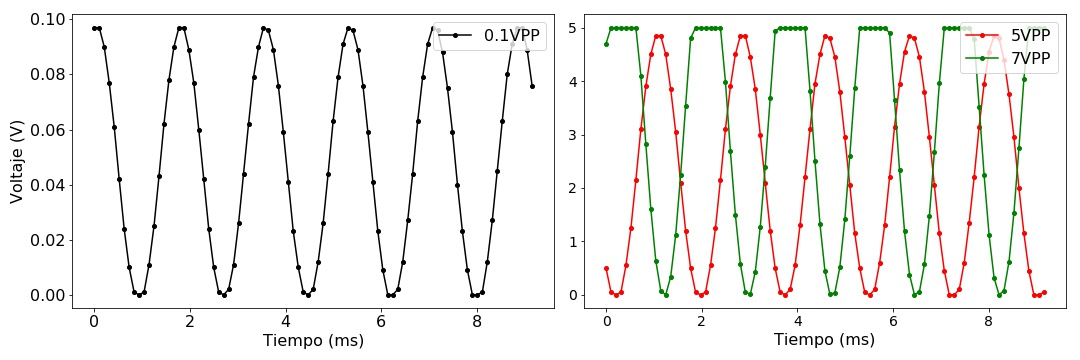
\includegraphics[width=\textwidth]{amplitud_arduino.jpg} \\
  (a) \hspace{4cm} (b)
  \caption{Respuesta en amplitud (a) mínima y (b) máxima de la placa arduino {\sc uno}.}
  \label{fig:amp-arduino}
\end{figure}

La respuesta en frecuencia de la placa arduino se puede ver en la Figura~\ref{fig:freq-arduino}. Los mediciones de frecuencia (Frecuencia de Salida) se realizaron variando la frecuencia de una onda sinusoidal (Frecuencia de Entrada) desde 1 a 700 Hz con el generador de onda. El incremento de las barras de error de nuestra medición muestra que la placa empieza a tener dificultades para detectar frecuencias mayores a ese valor. 
\begin{figure}[H]
  \centering
  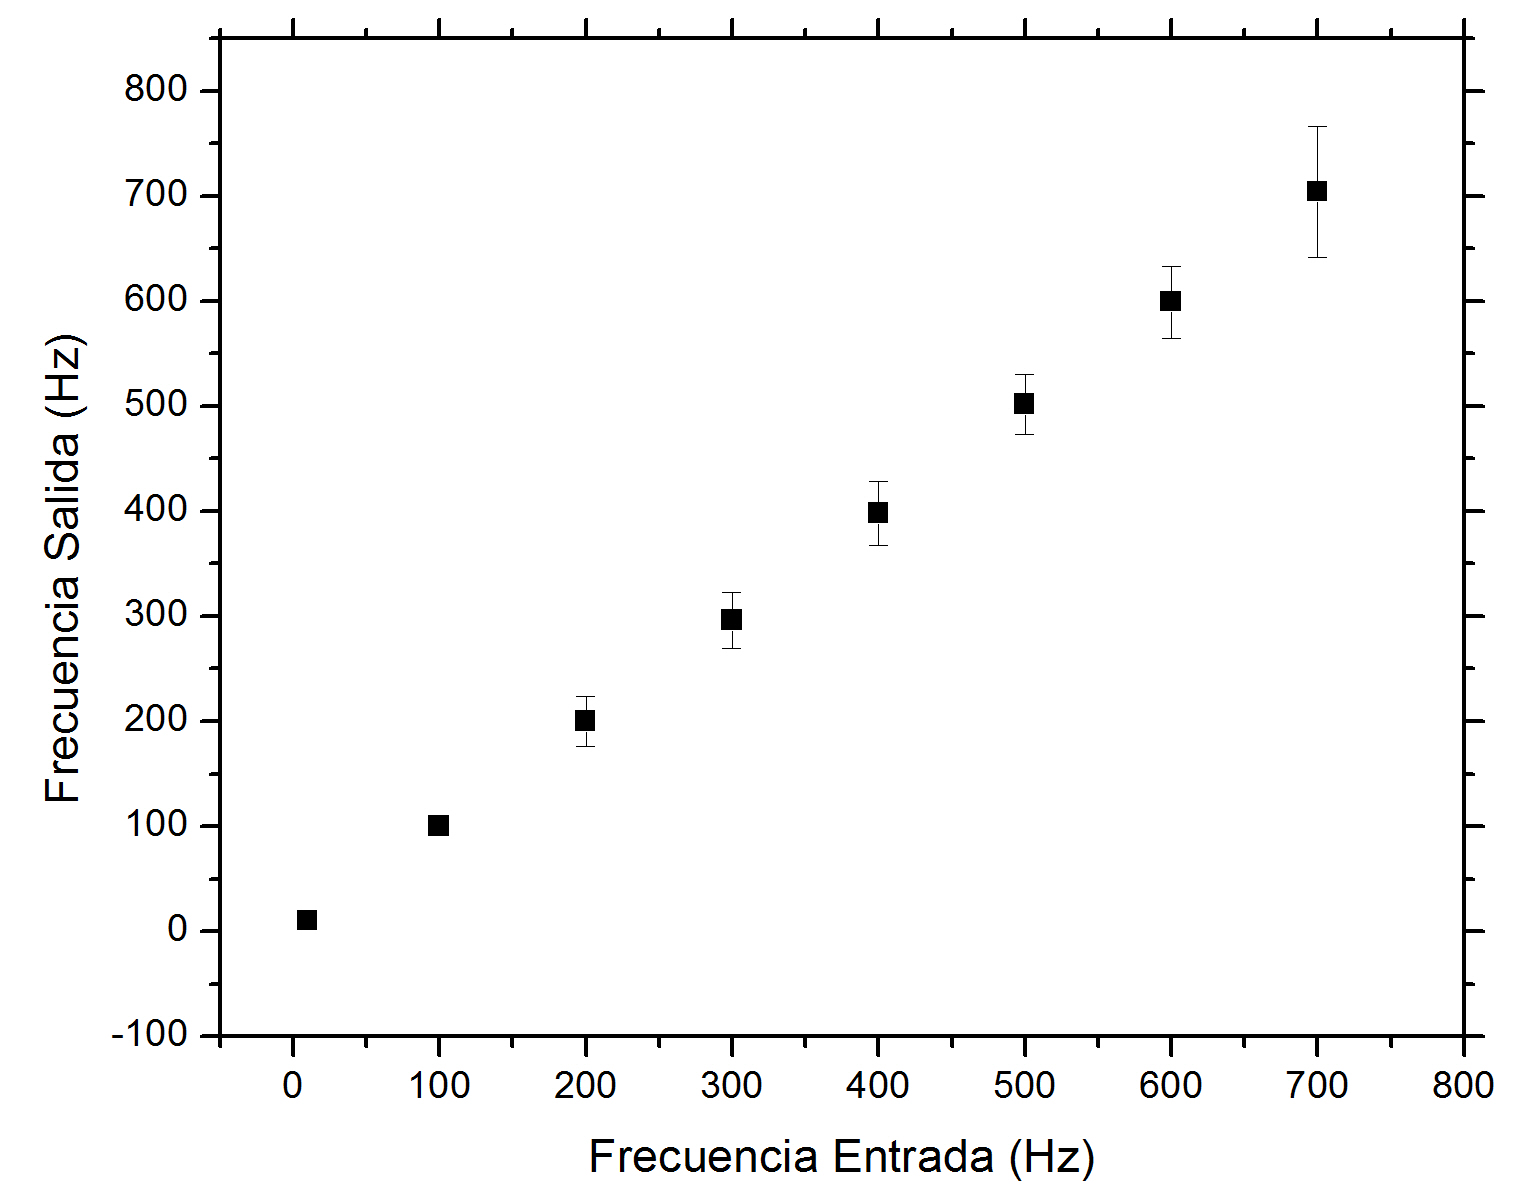
\includegraphics[width=0.6\textwidth]{FrecuenciasDelay100.jpg} \\
  (a) \hspace{4cm} (b)
  \caption{Respuesta en frecuencia de la placa arduino {\sc uno}.}
  \label{fig:freq-arduino}
\end{figure}

%Las limitaciones en respuesta de la placa arduino {\sc uno} se ven opacadas por la gran versatilidad en la recepción (y envío) de señales.

En la Tabla~\ref{tab:in-arduino} resumimos los datos recolectados en la caracterización de entrada de la placa.
\begin{table}[h]
\begin{tabularx}{\textwidth}{b|s|s|s }
Característica & Min & Máx & Unidad \\
\hline
Voltaje señal de entrada pin analógico & 0.1 & 5 & V \\ 
%Voltaje señal de salida pin digital & -5 & 5 & V \\
Frecuencia señal de entrada pin analógico & 10 & 700 & Hz \\
%Frecuencia señal de salida pi digital & 10 & 10000 & Hz 
\end{tabularx}
\label{tab:in-arduino}
\caption{Caracterización de señales de entrada de la placa de audio.}
\end{table}

\end{document}
